%!TEX root = ../master.tex

\chapter{Reinforcement Learning} % (fold)
	\label{cha:reinforcement_learning}


\section{Markov Reward and Decision Process} % (fold)
	\label{sec:markov_reward_and_decision_process}

	\subsection{State Value Function Closed-form} % (fold)
		\label{sub:state_value_function}
		
		For a Markov Reward Process ($\mathcal{S}, \mathcal{P}, \mathcal{R}, \gamma$), with 
		\begin{itemize}
			\item $\mathcal{S}$ the States
			\item $\mathcal{P}$ The transition matrix
			\item $\mathcal{R}$ the reward matrix
			\item $ \gamma $the discount
		\end{itemize}

		We define then the Return $\mathsf R_t$ and the State Value Function
		$\mathsf v (s) = \mathbb{E}[\mathsf R_t  S_t = s]$\\
		Then we have, in a vector form : 
		\[
			\mathbf{v} = (\mathbb{1} - \gamma \mathcal P )^{-1} \mathcal{R}
		\]
		Unfortunately, Matrix inversion in costly, so this is only feasible in small Markov Reward Process
	% subsection state_value_function (end)

	\subsection{Iterative Policy Evaluation Algorithm} % (fold)
		\label{sub:iterative_policy_evaluation_algorithm}

		In RL, we need not only the value of different state, but also a policy to define which action to take in any state. Then, we had an action space $\mathcal{A}$ and a policy $\pi$ to a MRP to obtaine what is called a Markov Decision Process	(MDP).

		The first algorithm is a method to evaluate a policy. We don't need to store all the previous value of V while updating, and furthermore, it converges faster this way.

		\begin{algorithm}[H]
				\KwData{a MDP ($\mathcal{S}$, $\mathcal{P}$, $\mathcal{A}$, $\mathcal{R}$, $\gamma$) and $\pi$ the policy to be evaluate }
				\KwResult{The value function $V^{\pi}$}
				Initialise V(s) =0 $\forall s$ \;
				\While{Convergence condition (number of epoch, $\Delta \leq$ threshold, ...)}
				{
					\ForAll{$s \in S$}
					{
						$v \leftarrow V(s)$ \;
						$V(s) \leftarrow \sum_\alpha \pi(s, \alpha) \sum_{s'} \mathcal{P}^a_{ss'}[\mathcal{R}^a_{ss'} + \gamma V(s')]$ \;
						$\Delta \leftarrow \max(\Delta, \abs{v - V(s)}) $ 
					}
				}
				Return V
				\caption{Iterative Policy Evaluation Algorithm}
			\end{algorithm}

	% subsection iterative_policy_evaluation_algorithm (end)
% section markov_reward_and_decision_process (end)

\section{Dynamic Programming in RL} % (fold)
	\label{sec:dynamic_programming_in_rl}

	In order to compute an optimal policy, we can do better than trying every policy and evaluating their $V^{\pi}$, the first class of algorithm enter in the Dynamic programming family. Convergence are assured by theorem relative to the Belmann equation (Policy Improvement theorem, Belmann principle of optimality, ...).
	\subsection{Policy Iteration Algorithm} % (fold)
		\label{sub:policy_iteration_algorithm}
		
		First algorithm simply apply a greedy \textbf{deterministic} policy relative to the Value function, and recalculate the new Value function, until the policy is stable (and according to theorem, optimal).


		\begin{algorithm}[H]
				\KwData{a MDP ($\mathcal{S}$, $\mathcal{P}$, $\mathcal{A}$, $\mathcal{R}$, $\gamma$)}
				\KwResult{The optimal policy $\pi*$ and his corresponding value function $V^{\pi*}$}
				Initialise V(s)=0 and $\pi(s) \in \mathcal{A},  \forall s$ \;
				\While{Convergence condition (policy is stable, or number of epoch)}
				{
					Do a Policy Evaluation for $\pi$ (with the Iterative Policy Evaluation for exemple)
					\ForAll{$s \in S$}
					{
						$b \leftarrow \pi(s)$ \;
						$\pi(s) \leftarrow \arg \max_a \sum_{s'} \mathcal{P}^a_{ss'}[\mathcal{R}^a_{ss'} + \gamma V(s')]$ \;
						$\text{policy-not-stable} \leftarrow (b \neq \pi(s) )\vee \text{policy-not-stable} $ 
					}
				}
				Return V
				\caption{Iterative Policy Evaluation Algorithm}
			\end{algorithm}

		This can be seen as the following scheme : 

		\begin{figure}[ht]
			\centering
			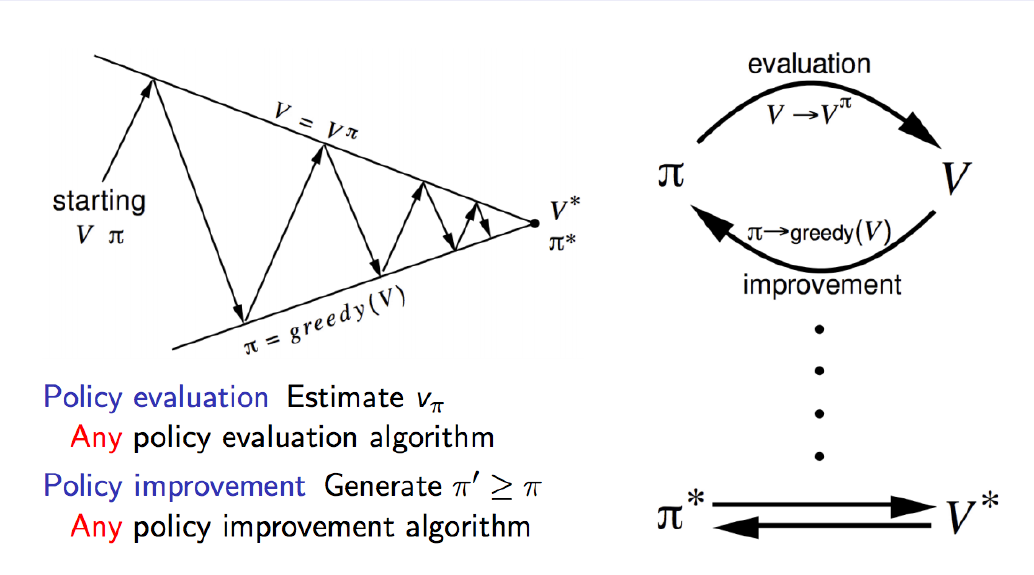
\includegraphics[scale=0.5]{figures/GenPolicyIteration}
			\caption{Generialised Policy Iteration Algorithm}
		\end{figure}
	% subsection value_iteration_algorithm (end)

	\subsection{Value Iteration Algorithm} % (fold)
		\label{sub:value_iteration_algorithm}
	
	% subsection policy_iteration_algorithm (end)

	\subsection{Assynchronous Backup in RL} % (fold)
		\label{sub:assynchronous_backup_in_rl}
		
		\paragraph{Prioritised Sweeping} % (fold)
			\label{par:prioritised_sweeping}
		
		% paragraph prioritised_sweeping (end)

		\paragraph{Real-time Dynamic Programming} % (fold)
			\label{par:real_time_dynamic_programming}
		
		% paragraph real_time_dynamic_programming (end)

	% subsection assynchronous_backup_in_rl (end)
	
	\subsection{Properties and drawbacks of Dynamic Programming} % (fold)
		\label{sub:properties_and_drawbacks_of_dynamic_programming}
	
	% subsection properties_and_drawbacks_of_dynamic_programming (end)

% section dynamic_programming_in_rl (end)

\section{Model-Free Learning} % (fold)
	\label{sec:model_free_learning}

	\subsection{Monte-Carlo Algorithms} % (fold)
		\label{sub:monte_carlo_algorithm}

		\paragraph*{(First Visit) Monte-Carlo Policy Evaluation}

		\paragraph*{Every Visit Monte-Carlo Policy Evaluation}

		\todo{Add "you cannot backup death" explanations}

		\paragraph*{Batch vs Online Monte-Carlo}

		\paragraph*{Incremental Monte-Carlo Update}

		\paragraph*{Runing Mean for Non-Stationnary World}
	% subsection monte_carlo_algorithms (end)

	\subsection{Monte-Carlo Control Algorithms} % (fold)
		\label{sub:monte_carlo_control_algorithms}
	
		\paragraph*{Monte-Carlo Policy Improvement}

			\subparagraph*{Greedy Policy Improvement over State Value Function}

			\subparagraph*{Greed Policy Improvement over State-Action Value Function}

		\paragraph*{Exploring Starts Problem}
			\todo{Don't forget Starting to explore}

		\paragraph*{On Policy Soft Control}
		
		\paragraph*{On-Policy $\epsilon$-greedy first-visit Monte-Carlo control Algorithm}

		\paragraph*{Monte-Carlo Batch Learning to Control}

		\paragraph*{Monte-Carlo Iterative Learning to Control}
	% subsection monte_carlo_control_algorithms (end)

	\subsection{Temporal Difference Learning} % (fold)
		\label{sub:temporal_difference_learning}
		
		\paragraph*{Temporal Difference Value Function Estimation Algorithm}
	% subsection temporal_difference_learning (end)
	\todo{Add Comparison between MC and TD learning}

	\subsection{Temporal Difference Learning Control Algorithm} % (fold)
		\label{sub:temporal_difference_learning_control_algorithm}
		
		\paragraph*{SARSA - On Policy learning Temporal Difference Control:}
			Here is the Sarsa Algorithm : \\
			\begin{algorithm}[H]
				\KwData{State $\mathcal{S}$, Action $\mathcal{A}$, Reward $\mathcal{R}$ and Discount $\gamma$}
				\KwResult{The optimal Q(S, A) State-Action Value Function and a greedy policy w.r.t Q}
				Initialise Q(s, a) $\forall a, s$ with Q(terminal state, a) = 0  \;
				\While{Convergence condition (number of epoch, $\Delta \leq$ threshold, ...)}
				{
					Initialise a state S\;
					Choose action A from S with $\epsilon$-greedy policy derived from Q\;
					\While{S is not a terminal State}
					{
						Take action A, observe reward R and next state S'\;
						Choose action A' from S' with $\epsilon$-greedy policy derived from Q\;
						Update $Q(S, A) \leftarrow Q(S, A) + \alpha (R + \gamma Q(S', A')- Q(S, A))$\;
						$S \leftarrow S', A \leftarrow A'$
					}
				}
				Return $Q$ and $\pi$ the derived policy
				\caption{SARSA algorithm with $\epsilon$-greedy policy}
			\end{algorithm}

			\begin{theorem}
				\textbf{Convergence of Sarsa} \\
				$Q(s, a) \rightarrow Q^\infty(s,a)$ under :
				\begin{itemize}
					\item GLIE (Greedy in the Limite with infinite exploration), which mean every state is visited infinitely many times and that the policy converge toward a greedy-policy (ex: $\epsilon$-greedy with $\epsilon\rightarrow 0$).
					\item Robbins-Monroe sequence of step-sizes $\alpha_t$ : which imply $\sum \alpha_t$ diverge and $\sum \alpha_t^2$ converge.
				\end{itemize}
			\end{theorem}
			\remark{the $\epsilon$-greedy policy can be replaced by any policy derived from Q. (Because Q is the one updated by the algorithm)}

			\subparagraph*{SARSA-Lambda}
			\subparagraph*{Hindsight Experience Replay}

		\paragraph*{Q-Learning: Off-Policy Temporal Difference Learning}

	% subsection temporal_difference_learning_control_algorithm (end)

% section model_free_learning (end)

\section{Reinforcement Learning with Function Approximation} % (fold)
	\label{sec:reinforcement_learning_with_function_approximation}

	\subsection{Exemple of features} % (fold)
		\label{sub:exemple_of_features}

		\paragraph*{Coarse Coding}
		\paragraph*{Tile Coding}
		\paragraph*{Radial-Basis Function}
		\paragraph*{Deep Learning}
	% subsection exemple_of_features (end)

	\subsection{Monte-Carlo with Value Function Approximation} % (fold)
		\label{sub:monte_carlo_with_value_function_approximation}
	
	% subsection monte_carlo_with_value_function_approximation (end)
	
	\subsection{Temporal Difference Learning with Value Function Approximation} % (fold)
	\label{sub:temporal_difference_learning_with_value_function_approximation}

	% subsection temporal_difference_learning_with_value_function_approximation (end)
	
	\subsection{Q-Learning with FA} % (fold)
	\label{sub:q_learning_with_fa}
	
	% subsection q_learning_with_fa (end)
	
	\subsection{subsection name} % (fold)
	\label{sub:subsection_name}
	
	% subsection subsection_name (end)
% section reinforcement_learning_with_function_approximation (end)

\section{Deep Learning Reinforcement Learning} % (fold)
	\label{sec:deep_learning_reinforcement_learning}

	\subsection{Experience Replay} % (fold)
		\label{sub:experience_replay}
	
	% subsection experience_replay (end)
	\subsection{Target Network} % (fold)
		\label{sub:target_network}
	
	% subsection target_network (end)
	\subsection{Clipping of Rewards} % (fold)
		\label{sub:clipping_of_rewards}
	
	% subsection clipping_of_rewards (end)
	\subsection{Skipping of Frames} % (fold)
	\label{sub:skipping_of_frames}
	
	% subsection skipping_of_frames (end)
% section deep_learning_reinforcement_learning (end)
% chapter reinforcement_learning (end)